%!TEX root = ../main.tex

We illustrate how \cosette can be used both for whole-program and compositional symbolic testing of JavaScript programs. We demonstrate how \cosette  explicitly exposes the resilience of JavaScript programs to the environment, not considered by standard symbolic execution tools, but essential for compositional analysis.

Our running example is a \emph{key-value map} implementation, given in Figure~\ref{fig:2a}. It contains four functions: 
\jsinline|Map|, for constructing an empty map;
\jsinline|get|, for retrieving the value associated with a given key;
\jsinline|put|, for inserting/updating key-value pairs; and \jsinline|validKey|, for deciding whether or not a key is valid.

 \begin{figure*}[t]
 \centering
 %
 \begin{subfigure}[b]{0.33\textwidth}
 {\lstset{language=JavaScript,basicstyle=\fontsize{7}{7}\ttfamily,escapeinside={~}{~}}
 \begin{lstlisting}
function Map () { this._contents = {} }

Map.prototype.get = function (k) {
  var c = this._contents;
  if this.validKey(k) {
    return (c.hasOwnProperty(k) ? c[k] : null)
  } else throw new Error("Invalid Key");
}

Map.prototype.put = function (k, v) {
  if this.validKey(k) {  
    this._contents[k] = v   
  } else throw new Error("Invalid Key");
} 

Map.prototype.validKey = function (k) { ... }
\end{lstlisting}}
\vspace*{-0.2cm}
\caption{Library implementation}
\label{fig:2a}
\end{subfigure}
%
 \begin{subfigure}[b]{0.33\textwidth}
 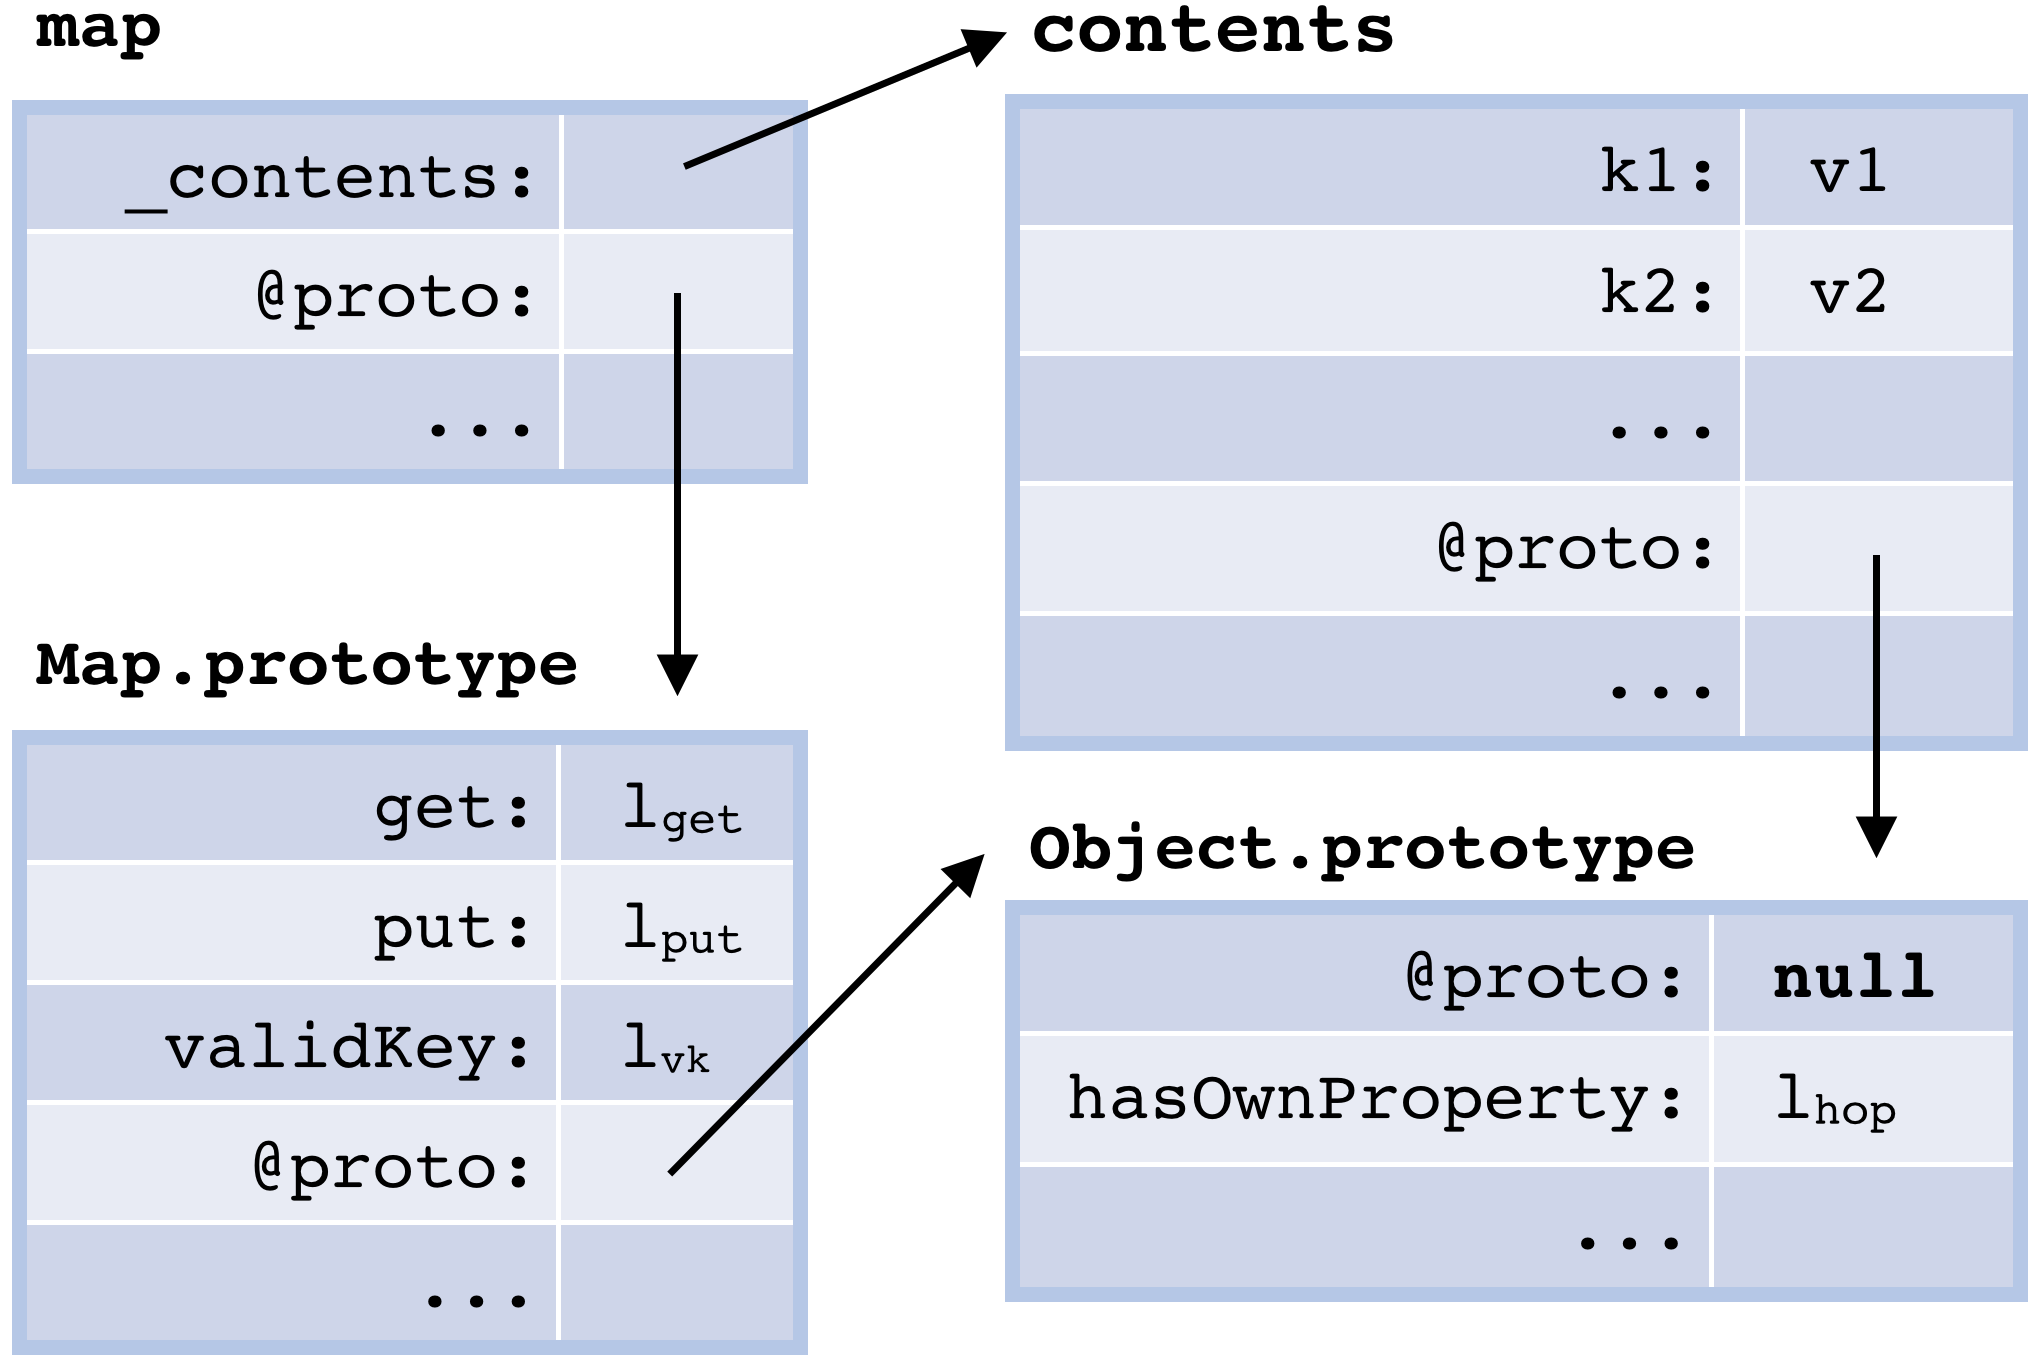
\includegraphics[width=0.93\textwidth]{figures/mapDiagram.png}
 \vspace*{0.5cm}
 \caption{General library heap}
 \label{fig:2b}
 \end{subfigure}
 %
 \begin{subfigure}[b]{0.3\textwidth}
 \centering 
 {\lstset{xleftmargin=.17\textwidth,language=JavaScript,basicstyle=\fontsize{7}{7}\ttfamily,escapeinside={~}{~}}
\begin{lstlisting}
var k = symb_string();
var v = symb_number();
assume(validKey(k));
var m = new Map(); m.put(k, v); 
var result = m.get(k);
assert(result = v)
\end{lstlisting}}
\vspace*{0.1cm}
 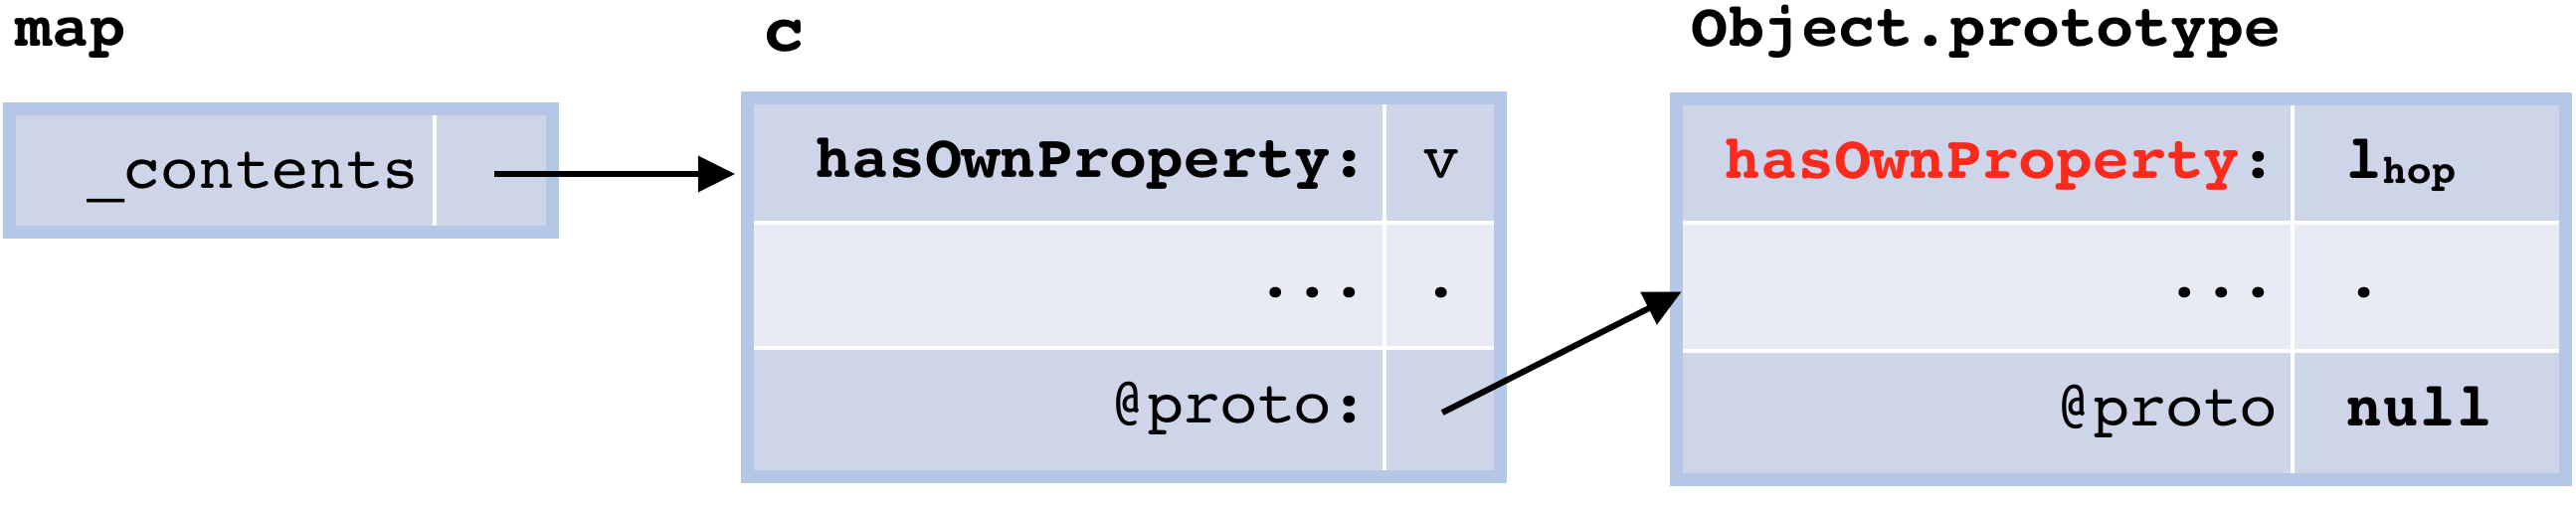
\includegraphics[width=0.78\textwidth]{figures/heapfail.png}
 \captionsetup{format=nastyCaption}
\caption{Simple symbolic test (above); \\the \jsinline|"hasOwnProperty"| bug (below)}
\label{fig:2c}
\end{subfigure}
\vspace*{-0.25cm}
\caption{Running example: JavaScript key-value map library}
\label{fig:two}
 \vspace*{-0.4cm}
\end{figure*}

\myparagraph{Description of the example}
The map library implements a \emph{key-value map} as an object with property \jsinline|_contents|, denoting the object storing the map contents.  
The named properties of \jsinline|_contents| and their value attributes correspond to the map keys and values, respectively.
The functions \jsinline|get|, \jsinline|put|, and \jsinline|validKey| are shared between all map 
objects and are, therefore, defined in \jsinline|Map.prototype|, which is the prototype\footnote{In JavaScript, inheritance is modelled through \emph{prototype chains}. On property lookup, $\mathtt{o.p}$, we first check if the property $\mathtt{p}$ is present in the object $\mathtt{o}$, in which case its value is returned. Otherwise, we  check if $\mathtt{p}$ is present in the prototype of $\mathtt{o}$, and so  forth.} of all objects created using \jsinline|Map| as a constructor (i.e.,~using~\jsinline|new Map()|). 
The \jsinline|get| function returns the value associated with a given key in the map, or \jsinline|null| if the key is not in the map. 
Note that, in order to check that the given key is in the map, \jsinline|get| uses the built-in function \jsinline|hasOwnProperty|, which lives in \jsinline|Object.prototype|, the prototype of all objects.
The \jsinline|put| function updates the map if the supplied key is valid, and otherwise throws an error. 
The \jsinline|validKey| function describes the conditions under which a given key is valid. 

In Figure \ref{fig:2b}, we show a general heap of key-value maps. There is the \jsinline|map| object, with its \jsinline|_contents| property pointing to the \jsinline|contents| object and its prototype being \jsinline|Map.prototype|. There is the \jsinline|contents| object, which holds the key-value pairs, and whose prototype is \jsinline|Object.prototype|. There is the \jsinline|Map.prototype| object, which holds the \jsinline|get|, \jsinline|put|, and \jsinline|validKey| functions,\footnote{In JavaScript, functions are modelled as objects in the heap. As their structure does not add to this example, we only show the locations of the appropriate objects.} and whose prototype is also \jsinline|Object.prototype|. Finally, there is \jsinline|Object.prototype|, which holds the \jsinline|hasOwnProperty| function that is called by \jsinline|Map.prototype.get|.

%Observe that a naive implementation of the function \jsinline|validKey| may result in potential bugs. In particular, one can insert a key-value pair with \jsinline|"hasOwnProperty"| as a key into the map. By doing this, \jsinline|"hasOwnProperty"| in the prototype chain of \jsinline|_contents| is overridden and subsequent calls to \jsinline|get| will fail. 

%\myparagraph{Prototype chains and $\mathtt{Object.prototype}$}
%In order to better understand the implementation of the map library as well as its possible bugs, 
%one must first understand the \emph{prototype-based inheritance} mechanism of JavaScript. 
%Every JavaScript object has a prototype, which (for presentation purposes) we assume to 
%be stored  in an internal property \jsinline|@proto|. In order to determine the value of a property
%\jsinline|p| of an object \jsinline|o|, the semantics first checks if \jsinline|o| has a 
%property named \jsinline|p|, in which case the property look-up yields its value. Otherwise, the 
%semantics checks if \jsinline|p| belongs to the properties of the prototype of \jsinline|o| and so 
%forth. Hence, in the example, when looking up the value of the property \jsinline|hasOwnProperty|
%of the object \jsinline|contents|, one gets the value associated with the property  \jsinline|hasOwnProperty|
%of its prototype.
%The sequence of objects that can be accessed from a given object through the inspection 
%of the respective prototypes is called a \emph{prototype chain}.
%Prototype chains typically finish with the object \jsinline|Object.prototype| from which JavaScript 
%programs can access a number of built-in functions, which are part of the language runtime environment and are used for inspecting and manipulating objects.
%An example of such a function is \jsinline|hasOwnProperty(p)|, which checks whether or not the object 
%on which it is invoked has the property \jsinline|p| (e.g. {\small \jsinline|map.hasOwnProperty("_contents")|}
%evaluates to \jsinline|true| when evaluated in the heap shown in Fig.~\ref{map:example}-(right), 
%because the object \jsinline|map| has a property named~\jsinline|"_contents"|). 

\lstnewenvironment{lstjsex}{\lstset{language=JavaScript,basicstyle=\fontsize{8}{8}\ttfamily,escapeinside={~}{~}, numbers=none}}{}

\vspace*{-0.2cm}
\subsection{Whole-program Symbolic Testing}
\label{subsec:st}

Developers are used to writing unit tests for their code---verifying that, given some concrete inputs, the code produces the expected outputs. Using \cosette, they can write unit tests with \emph{symbolic} inputs and outputs, systematically testing a broad range of behaviours with a single symbolic test. For example, one meaningful unit test for the \jsinline|put| function consists of inserting a valid key-value pair \jsinline|(k, v)| into a map and then verifying that the pair has been inserted correctly. In Cosette, this test can be written as in Figure~\ref{fig:2c}. First, we declare \jsinline|k| to be a symbolic string and \jsinline|v| to be an symbolic number, using \cosette's constructs for creating symbolic variables. Next, we assume that \jsinline|k| is a valid key. Next, we create a new map, put the (symbolic) key-value pair \jsinline|(k, v)| into the map and then retrieve the value corresponding to the key~\jsinline|k|. Finally, we assert that the retrieved value is equal to the one we had previously put.

% 
When running \cosette on this test, if the \jsinline|validKey(k)| function was implemented incorrectly,\footnote{For instance, $\mathtt{validKey(k)}$ may only require that $\mathtt{k}$ is a string, which is a reasonable implementation, in the sense that it disallows JavaScript's implicit coercions.}
we will obtain the counter-model \jsinline|k = "hasOwnProperty"|. To understand this error, recall the heap and the implementation of \jsinline|get| from Figure~\ref{fig:two}. We can see that, if we were to put the key \jsinline|"hasOwnProperty"| into the contents object of a map, then the lookup of \jsinline|c.hasOwnProperty| done by \jsinline|get| will not reach \jsinline|Object.prototype| as intended, resolving instead to the \jsinline|hasOwnProperty| property of the contents object (Figure~\ref{fig:2c}, below).

This example highlights how \cosette does not require specialist knowledge and can 
be used as a testing tool by a general JavaScript developer. The annotations amount to the creation of 
symbolic variables and the writing of assumptions and assertions, remaining minimal and intuitive, in contrast with the standard annotation burden of verification tools.

\vspace*{-0.2cm}
\subsection{Specification-driven Bug-finding}
\label{subsec:sdbf}

%\pmax{
%\begin{itemize}
%\item Compositionality = resilience to frame
%\item Summaries have to be resilient to frame
%\item BUT there are also NONES, and this is what is new
%\item Now guide through
%\item POINT - resilient to ALL frames, for whole-program analysis we are resilient only to one frame - we do get to create it, but it's only one after all
%\item Then, we can have more general specs, but needn't necessarily
%\end{itemize}
%}

As well as for whole-program analysis, \cosette can be used for compositional symbolic analysis of JavaScript functions in isolation, where the user specifies the functions in terms of its pre- and post-conditions. These specifications may account for only the parts of the heap required for running the function and can involve predicates, both recursive and non-recursive. We deal with recursive predicates by unfolding them to a  bound specified by the user.

Much like symbolic tests generalise concrete tests, specifications generalise symbolic tests. Given a JavaScript function, its specification, and the unfold depth for predicates, \cosette generates symbolic tests to verify that the function conforms to the specification up to that given depth. If this is not the case, \cosette will return a concrete counter-model that invalidates the specification. Unlike whole-program analysis tools, \cosette also tests if the given specification is compositional, that is, if it is resilient against all possible contexts in which the function can be run, and reports back to the user any found sources of non-compositionality.

\cosette supports the specification of symbolic states via simple separation logic assertions in the style of JaVerT~\cite{javert}. The developer has at their disposal a number of built-in predicates that capture the fundamental concepts of JavaScript (discussed throughout the text), and can define their own predicates as well. For instance, learning from the previous symbolic test, we could define the following predicate for describing valid keys:
\begin{Verbatim}[fontsize=\footnotesize,commandchars=\\\{\}]
    ValidKey(k) := types(k : Str) * (k <> "hasOwnProperty"),
\end{Verbatim}
\noindent meaning that \jsinline|k| is a valid key if it is a string that is not equal to \jsinline|"hasOwnProperty"|. From there, if we wanted to do a full functional correctness specification of the \jsinline|Map| library, we could, guided by the heap in Figure~\ref{fig:2b}, define the following two predicates:

% \textcolor{red}{(m, "get") -> None * (m, "put") -> None * (m, "validKey") -> None} * 
% * NoProps(c, keys)

\smallskip
\begin{Verbatim}[fontsize=\footnotesize,commandchars=\\\{\}]
 Map (m, mp, kvs) := JSObjectWithProto(m, mp) * 
   DataProp(m, "_contents", c) * JSObject(c) * KVPairs(c, kvs) * 
     \textcolor{red}{NoProp(m, "get")} * \textcolor{red}{NoProp(m, "put")} * \textcolor{red}{NoProp(m, "validKey")} * 
       \textcolor{blue}{NoProps(c, FProj(kvs))}
\end{Verbatim}
\begin{Verbatim}[fontsize=\footnotesize,commandchars=\\\{\}]
  KVPairs (c, kvs) := (kvs = \{ \}),
                      (kvs = \{(k, v)\} U kvs') * ValidKey(k) * 
                        DataProp(c, k, v) * KVPairs(c, kvs')
\end{Verbatim}

\smallskip
The \jsinline|Map| predicate states that a map object is a standard JavaScript object with a given prototype \jsinline|mp|, and that it has the property \jsinline|_contents|, which points to a  JavaScript object \jsinline|c|.
Using the \jsinline|KVPairs| predicate, % (explained shortly), 
it also states that \jsinline|c| holds the key-value pairs \jsinline|kvs|. 
%Finally, it obtains the set of keys \jsinline|keys| from the set of key-value pairs using the first projection predicate \jsinline|First|, and then, using the \jsinline|NoProps| predicate, states that all other properties are absent from \jsinline|c|.
The \jsinline|KVPairs(c, kvs)| predicate is defined recursively: \jsinline|kvs| is either empty or contains at least one key-value pair \jsinline|(k, v)|, 
in which case we state that the key \jsinline|k| must be valid, that object \jsinline|o| has  property \jsinline|k| with value \jsinline|v|, and proceed recursively.
The highlighted parts of \jsinline|Map| describe the compositionality requirements: in red, we state that map objects must not have the properties \jsinline|"get"|, \jsinline|"put"|, and \jsinline|"validKey"|; in blue, we state that the object~\jsinline|c| has no other properties except for the map keys.\footnote{$\mathtt{NoProp(o, p)}$  states that the object $\mathtt{o}$ does not have property $\mathtt{p}$; $\mathtt{NoProps(o, props)}$ states that the object $\mathtt{o}$ has no properties outside of those from the set $\mathtt{props}$; the $\mathtt{FProj}$ operator extracts the set of keys from the set of key-value pairs.}
%
%The uniqueness of keys is guaranteed by the \jsinline|DataProp| predicate of \jsinline|KVPairs| and the separating conjunction.
We also require a \jsinline|MapProto(mp)| predicate, describing that \jsinline|mp| is a valid map prototype, that is, that it defines the \jsinline|put|, \jsinline|get|, and \jsinline|validKey| methods. To avoid clutter, we keep its definition opaque.

\begin{wrapfigure}{R}{0.23\textwidth}
\vspace*{-0.3cm}
\hspace*{-0.8cm}
$
{\scriptsize
\begin{array}{c}
\left\{ {\begin{array}{c}
 \text{\texttt{Map(m, mp, kvs) * MapProto(mp) *}} \\
 \text{\texttt{ValidKey(k) * (k $\notin$ FProj(kvs)) *}} \\
 \text{\textcolor{blue}{\texttt{Writable(Object.prototype, k)}}}
\end{array}} \right\} \\
%
\text{\bfseries \texttt{m.put(k, v)}} \\[0.2mm]
%
\left\{ {\begin{array}{c}
 \text{\texttt{Map(m, kvs -u- (k, v)) * MapProto(mp) *}} \\
 \text{\textcolor{blue}{\texttt{Writable(Object.prototype, k)}}} \\
\end{array}} \right\}
\end{array}
} 
$
\vspace*{-0.4cm}
\end{wrapfigure}

On the right, we show one compositional specification of \jsinline|put(k, v)|. 
We assume a map object \jsinline|m|, with key-value pairs \jsinline|kvs| and prototype \jsinline|Map.Prototype|. We also assume that \jsinline|k| is a valid key not already in the map. For compositionality, highlighted in blue, we have to state that the property \jsinline|k| is not non-writable in \jsinline|Object.prototype|.\footnote{In JavaScript, object properties can be non-writable, meaning that their value cannot be changed. In this specification, we assume that the property exists and is writable. There is an analogous specification for $\mathtt{put}$, in which the property does not exist.}
In the end, the key-value pair has been inserted into the map, while the remaining part of the heap remains unchanged.

% for example, \jsinline|JSObject(o)| states that \jsinline|o| is a standard JavaScript object; \jsinline|JSObjectWithProto(o, op)| states that \jsinline|o| is a JavaScript object with prototype \jsinline|op|; and \jsinline|DataProp(o, p, v)| states that the property \jsinline|p| of~\jsinline|o| has value \jsinline|v|. One can also describe the absence of object properties: \jsinline|NoProp(o, p)| states that the object~\jsinline|o| does not have property \jsinline|p|, and \jsinline|NoProps(o, props)| states that the object \jsinline|o| has no other properties except those in the set \jsinline|props|. There also exist predicates for describing function objects, prototype chains, function closures, etc.,

%\smallskip
%\begin{minipage}{0.475\textwidth}
%\begin{displaymath} 
%{\scriptsize
%\begin{array}{c}
%\left\{ {\begin{array}{c}
% \text{\texttt{Map(m, mp, kvs -u- (k, v')) * MapProto(mp)}}
%\end{array}} \right\} \\
%%
%\text{\bfseries \texttt{m.put(k, v)}} \\[0.2mm]
%%
%\left\{ {\begin{array}{c}
% \text{\texttt{Map(m, kvs -u- (k, v)) * MapProto(mp)}}
%\end{array}} \right\}
%\end{array}
%} 
%\end{displaymath}
%\end{minipage}
%\quad
%\begin{minipage}{0.48\textwidth}
%%
%\begin{displaymath} 
%{\scriptsize
%\begin{array}{c}
%\left\{ {\begin{array}{c}
% \text{\texttt{Map(m, mp, kvs) * MapProto(mp) *}} \\
% \text{\texttt{ValidKey(k) * (k $\notin$ First(kvs))}}
%\end{array}} \right\} \\
%%
%\text{\bfseries \texttt{m.put(k, v)}} \\[0.2mm]
%%
%\left\{ {\begin{array}{c}
% \text{\texttt{Map(m, kvs -u- (k, v)) * MapProto(mp)}}
%\end{array}} \right\}
%\end{array}
%} 
%\end{displaymath}
%\end{minipage}

%\pmax{Explain specs a bit}

When symbolically testing the specifications of the \jsinline|Map| library functions, the \jsinline|"hasOwnProperty"| bug will not be triggered again, as \jsinline|ValidKey(k)| has been adjusted appropriately. However, if we were to forget the highlighted parts in the \jsinline|Map| definition and \jsinline|put| specification, we would encounter other issues, exposing the tension between compositionality and dynamic languages. 

\begin{wrapfigure}{R}{0.18\textwidth}
\vspace*{-0.4cm}
\hspace*{-0.6cm}
\centering
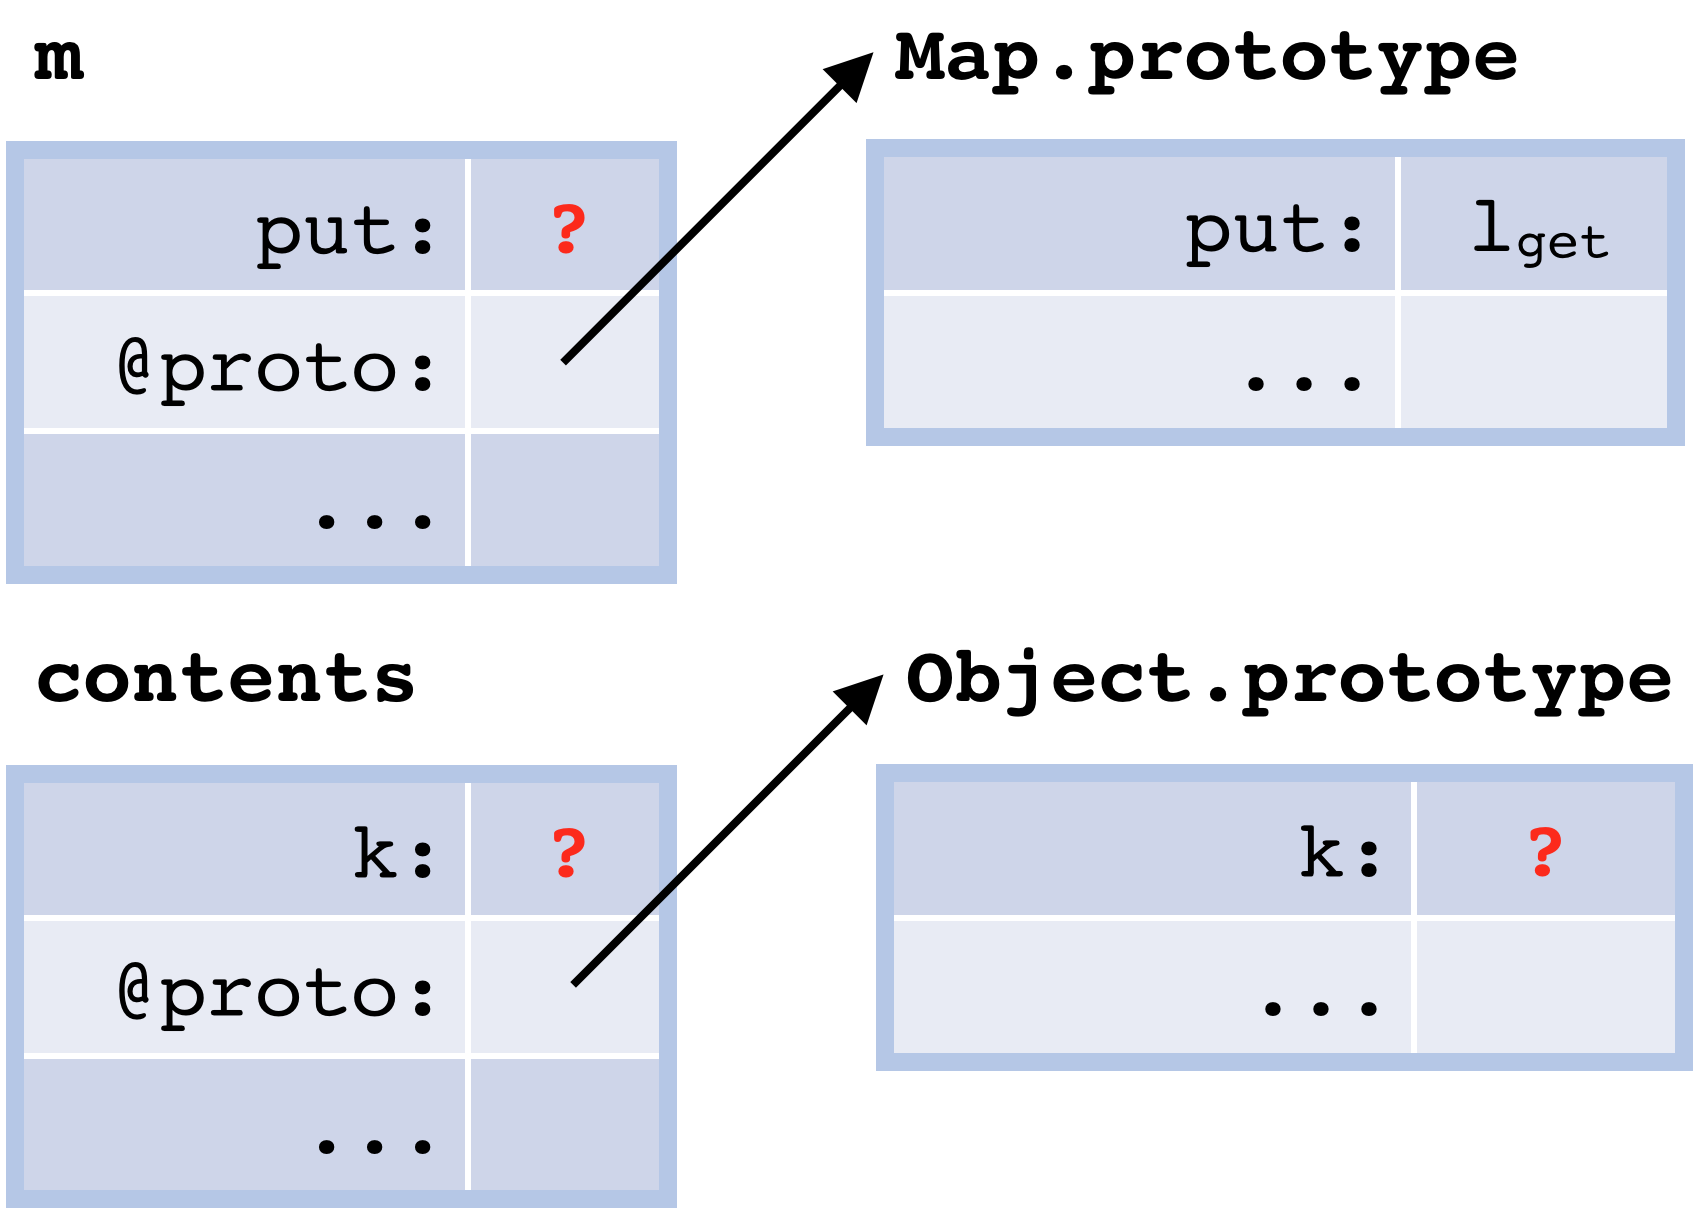
\includegraphics[width=0.21\textwidth]{figures/compositional.png}
\vspace*{-0.58cm}
\caption*{\hspace*{-0.58cm}{\small Figure 2. Compositionality}}
\vspace*{-0.4cm}
\end{wrapfigure}

\setcounter{figure}{2} 
First, if we omitted the part of the \jsinline|Map| predicate highlighted in red, \cosette would complain, when testing the \jsinline|put| function, that it has no information about the property \jsinline|"put"| of the map object~\jsinline|m| and cannot perform the lookup \jsinline|m.put| (Fig.~2, above). This means that the library code is not resilient to frames in which a map object \jsinline|m| has the property \jsinline|put|.
Analogous issues would arise for the \jsinline|"get"| and \jsinline|"validKey"| properties.% which also must be absent from all map objects. 

Second, if we omitted the parts highlighted in blue, upon execution of the line \jsinline|this._contents[k] = v| (Fig.~\ref{fig:2a}, line 12) \cosette would complain that it has no information about the property \jsinline|k| in the prototype chain of the contents object (Fig.~2, below). This is required as the semantics of JavaScript has to look up the value of the property \jsinline|k| of the contents object before performing the actual assignment, to check if the assignment is allowed (i.e.,~ that the property is non-writable). As \jsinline|k| is symbolic, what this means is that the library is not resilient to frames in which there are non-writable properties in \jsinline|Object.prototype|. A similar issue arises for the \jsinline|Map| constructor (Fig.~\ref{fig:2a}, line 1), which requires the property \jsinline|"_contents"| not to be non-writable in the prototype chains of map objects.

%Now, we can give the complete definition of the \jsinline|Map| predicate and the corrected, compositional specification of \jsinline|put(k, v)| when \jsinline|k| is a valid key that is not in the map, with the compositionality-related changes highlighted in red:
%
%\noindent
%\begin{minipage}{0.58\textwidth}
%\begin{Verbatim}[fontsize=\footnotesize,commandchars=\\\{\}]
%  Map (m, mp, kvs) := 
%    JSObjectWithProto(m, mp) * \textcolor{red}{NoProp(m, "get")} * 
%    \textcolor{red}{NoProp(m, "put")} * \textcolor{red}{NoProp(m, "validKey")} * 
%    DataProp(m, "_contents", c) * JSObject(c) *
%    KVPairs(c, kvs) * \textcolor{red}{First(kvs, keys)} * \textcolor{red}{NoProps(c, keys)}
%\end{Verbatim} 
%\end{minipage}
%\begin{minipage}{0.42\textwidth}
%%
%\begin{displaymath} 
%{\scriptsize
%\begin{array}{c}
%\left\{ {\begin{array}{c}
% \text{\texttt{Map(m, mp, kvs) * MapProto(mp) *}} \\
% \text{\texttt{ValidKey(k) * (k $\notin$ First(kvs)) *}} \\
% \text{\textcolor{red}{\texttt{Writable(Object.prototype, k)}}}
%\end{array}} \right\} \\
%%
%\text{\bfseries \texttt{m.put(k, v)}} \\[0.2mm]
%%
%\left\{ {\begin{array}{c}
% \text{\texttt{Map(m, kvs -u- (k, v)) * MapProto(mp) *}} \\
% \text{\textcolor{red}{\texttt{Writable(Object.prototype, k)}}} \\
%\end{array}} \right\}
%\end{array}
%} 
%\end{displaymath}
%\end{minipage}

What this example illustrates is that, in order to be compositional, specifications of programs written in dynamic languages have to explicitly state which parts of the heap must not be present. \cosette is able to detect and report compositionality-related issues, such as those presented above, which are highly likely to remain unnoticed in whole-program analysis, as there we always have complete information about the entire contents of the heap.

%\subsection{Compositional Symbolic Testing}
%
%%\begin{wrapfigure}{R}{0.45\textwidth}
%%\vspace*{-0.5cm}
%%\centering
%%\begin{lstjsex}
%%[ Map(m, mp) * MapProto(mp) * ValidKey(k) ]
%%    m.put(k, v); 
%%    var result = m.get(k);
%%[ Precondition * (result = v) ]
%%\end{lstjsex}
%%\vspace*{-0.4cm}
%%\caption{Revisited test for \jsinline|Map|}
%%\label{test:map:2}
%%\vspace*{-0.35cm}
%%\end{wrapfigure}
%
%A general developer can write concrete and symbolic tests for their code, but cannot be expected to write full functional correctness specifications in separation logic. Using \cosette, they can combine the best of both worlds by describing only the shape of their \polish{heap/memory/data structure} using separation logic and then testing the behaviour of the code using symbolic tests. Using this approach, one can not only find the same bugs as in whole-program symbolic testing, but also detect compositionality issues triggered by the tests. 



%Refer to Figure 2 - the developer knows the heap and can describe it easily. If they forget, . Ideally, this would be automatic.
%
%We illustrate the compositional symbolic execution of \cosette using the \jsinline|get(k)| function of the key-value map example. Below, we revisit the code of \jsinline|get| and describe the heap before and after \jsinline|get(k)| is called with a valid key that is in the map. In order to do this, the developer needs to know the structure of the heap (Figure~\ref{map:example}) and use the built-in predicates.
%
%\smallskip
%\begin{minipage}{0.52\textwidth}
% \begin{lstjs}
%Map.prototype.get = function (k) {
%  var c = this._contents;
%  if this.validKey(k) {
%    return (c.hasOwnProperty(k) ? 
%               c[k] : null)
%  } else throw new Error("Invalid Key");
%}
%\end{lstjs}
%\end{minipage}
%\begin{minipage}{0.47\textwidth}
%$
%{\scriptsize
%\begin{array}{c}
%\left\{{\begin{array}{c}
% \text{\texttt{JSObjectWithProto(this, mp) * MapProto(mp) * }} \\
% \text{\texttt{DataProp(m, "\_contents", c) * JSObject(c) * }} \\
% \text{\texttt{ValidKey(k) * \color{blue}{DataProp(c, k, v)}}}
%\end{array}}\right\} \\
%%
%\text{\bfseries \texttt{get(k)}} \\
%%
%\left\{ {\begin{array}{c}
% \text{\texttt{StartingState * (ret = v)}} 
%\end{array}} \right\}
%\end{array}
%}
%$
%\end{minipage}
%
%\smallskip
%To describe the starting state, we first note that the map object on which \jsinline|get| was called has prototype \jsinline|mp|, representing \jsinline|Map.prototype|.\footnote{Some stuff.} Next, we state that the map object itself has property \jsinline|"_contents"| pointing to a standard JavaScript object \jsinline|c|, that the key \jsinline|k| is valid, and that the object \jsinline|c| has the property \jsinline|k| with value \jsinline|v|. In the final state, we additionally know that the return value of the function should be equal to \jsinline|v|.
%
%
%
%
%
%\vspace*{5cm}
%catch how the spec is not compositional, reveal frame non-resilience shit
%
%It is meant to be run as a method call, the this, it is in the prototype. validKey is also meant to be in the prototype. Refer to figure 2. the this has the contents field, then that is an object, the key k is valid and then it may or may not have the k field.
%
%Now, frame bugs will pop up and you will see how the function is not resilient to the frame.
%
%you can catch these bugs in real-world tests
%
%...and if they want, they can write a more general abstraction of the entire data structure, which may be recursive or not, then ask for it to be unfolded to a given depth and create symbolic tests from that.
%
%
%
%\newpage
%In order for a specification of a program to be compositional, it must be resilient against all the possible frames, that is, all possible contexts in which the program can be run. This is in contrast to whole-program analysis, which considers only one frame at a time. 
%
%we demonstrate how \cosette explicitly exposes the resilience of JavaScript programs to the environment, not  considered by standard symbolic execution tools, but essential for compositional analysis. Therefore, this .
%
%For that, we revisit the \javert specification of key-value maps. This specification involves several predicates, shown below, which use JavaScript-specific abstractions that hide the internals of the language, such as \jsinline|JSObject(c)|, which states that \jsinline|c| is a standard JavaScript object, and \jsinline|DataProp(o, p, v)|, which states that the property \jsinline|p| of \jsinline|o| has value \jsinline|v|.
%
%% \textcolor{red}{(m, "get") -> None * (m, "put") -> None * (m, "validKey") -> None} * 
%
%\begin{Verbatim}[fontsize=\footnotesize,commandchars=\\\{\}]
%    Map (m, kvs) := DataProp(m, "_contents", c) * JSObject(c) * 
%                      KVPairs(c, kvs) * first(kvs, keys) * emptyFields(c, keys)
%\end{Verbatim}
% \begin{Verbatim}[fontsize=\footnotesize,commandchars=\\\{\}]
%KVPairs (o, kvs) := (kvs = \{ \}),
%                    (kvs = (k, v) -u- kvs') * ValidKey(k) * DataProp(o, k, v) * KVPairs(o, kvs')
%\end{Verbatim}
%\begin{Verbatim}[fontsize=\footnotesize,commandchars=\\\{\}]
%    ValidKey (k) := types(k : Str) * \textcolor{red}{(k <> "hasOwnProperty")}
%\end{Verbatim}
%
%
%Refer to Figure 2 - the developer knows the heap and can describe it easily. If they forget, . Ideally, this would be automatic.
%
%The \jsinline|Map| predicate captures the resource corresponding to a map object. 
%Concretely, it first states that the map object has the property \jsinline|_contents|, which points to a  JavaScript object \jsinline|c|.
%Next, using the \jsinline|KVPairs| predicate (explained shortly), it states that \jsinline|c| holds the key-value pairs \jsinline|kvs|. Finally, it obtains the set of keys \jsinline|keys| from the set of key-value pairs using the first projection predicate \jsinline|first|, and then, via the \jsinline|emptyFields| assertion, states that all other properties are absent from \jsinline|c|.
%
%The \jsinline|KVPairs(o, kvs)| predicate talks about key-value pairs of an object \jsinline|o|. 
%It is defined recursively on the structure of \jsinline|kvs| and it has two definitions, separated by a comma. 
%We have that \jsinline|kvs| is either empty or that it contains at least one key-value pair \jsinline|(k, v)|,\footnote{We write $\mathtt{-u-}$ for set union and omit the brackets around singleton sets.} 
%in which case we state that the key \jsinline|k| must be valid, that object \jsinline|o| has  property \jsinline|k| with value \jsinline|v|, and proceed recursively.
%The uniqueness of keys is guaranteed by the \jsinline|DataProp| predicate of \jsinline|KVPairs| and the separating conjunction.
%
%\begin{wrapfigure}{R}{0.3\textwidth}
%\vspace*{-0.45cm}
%\centering
%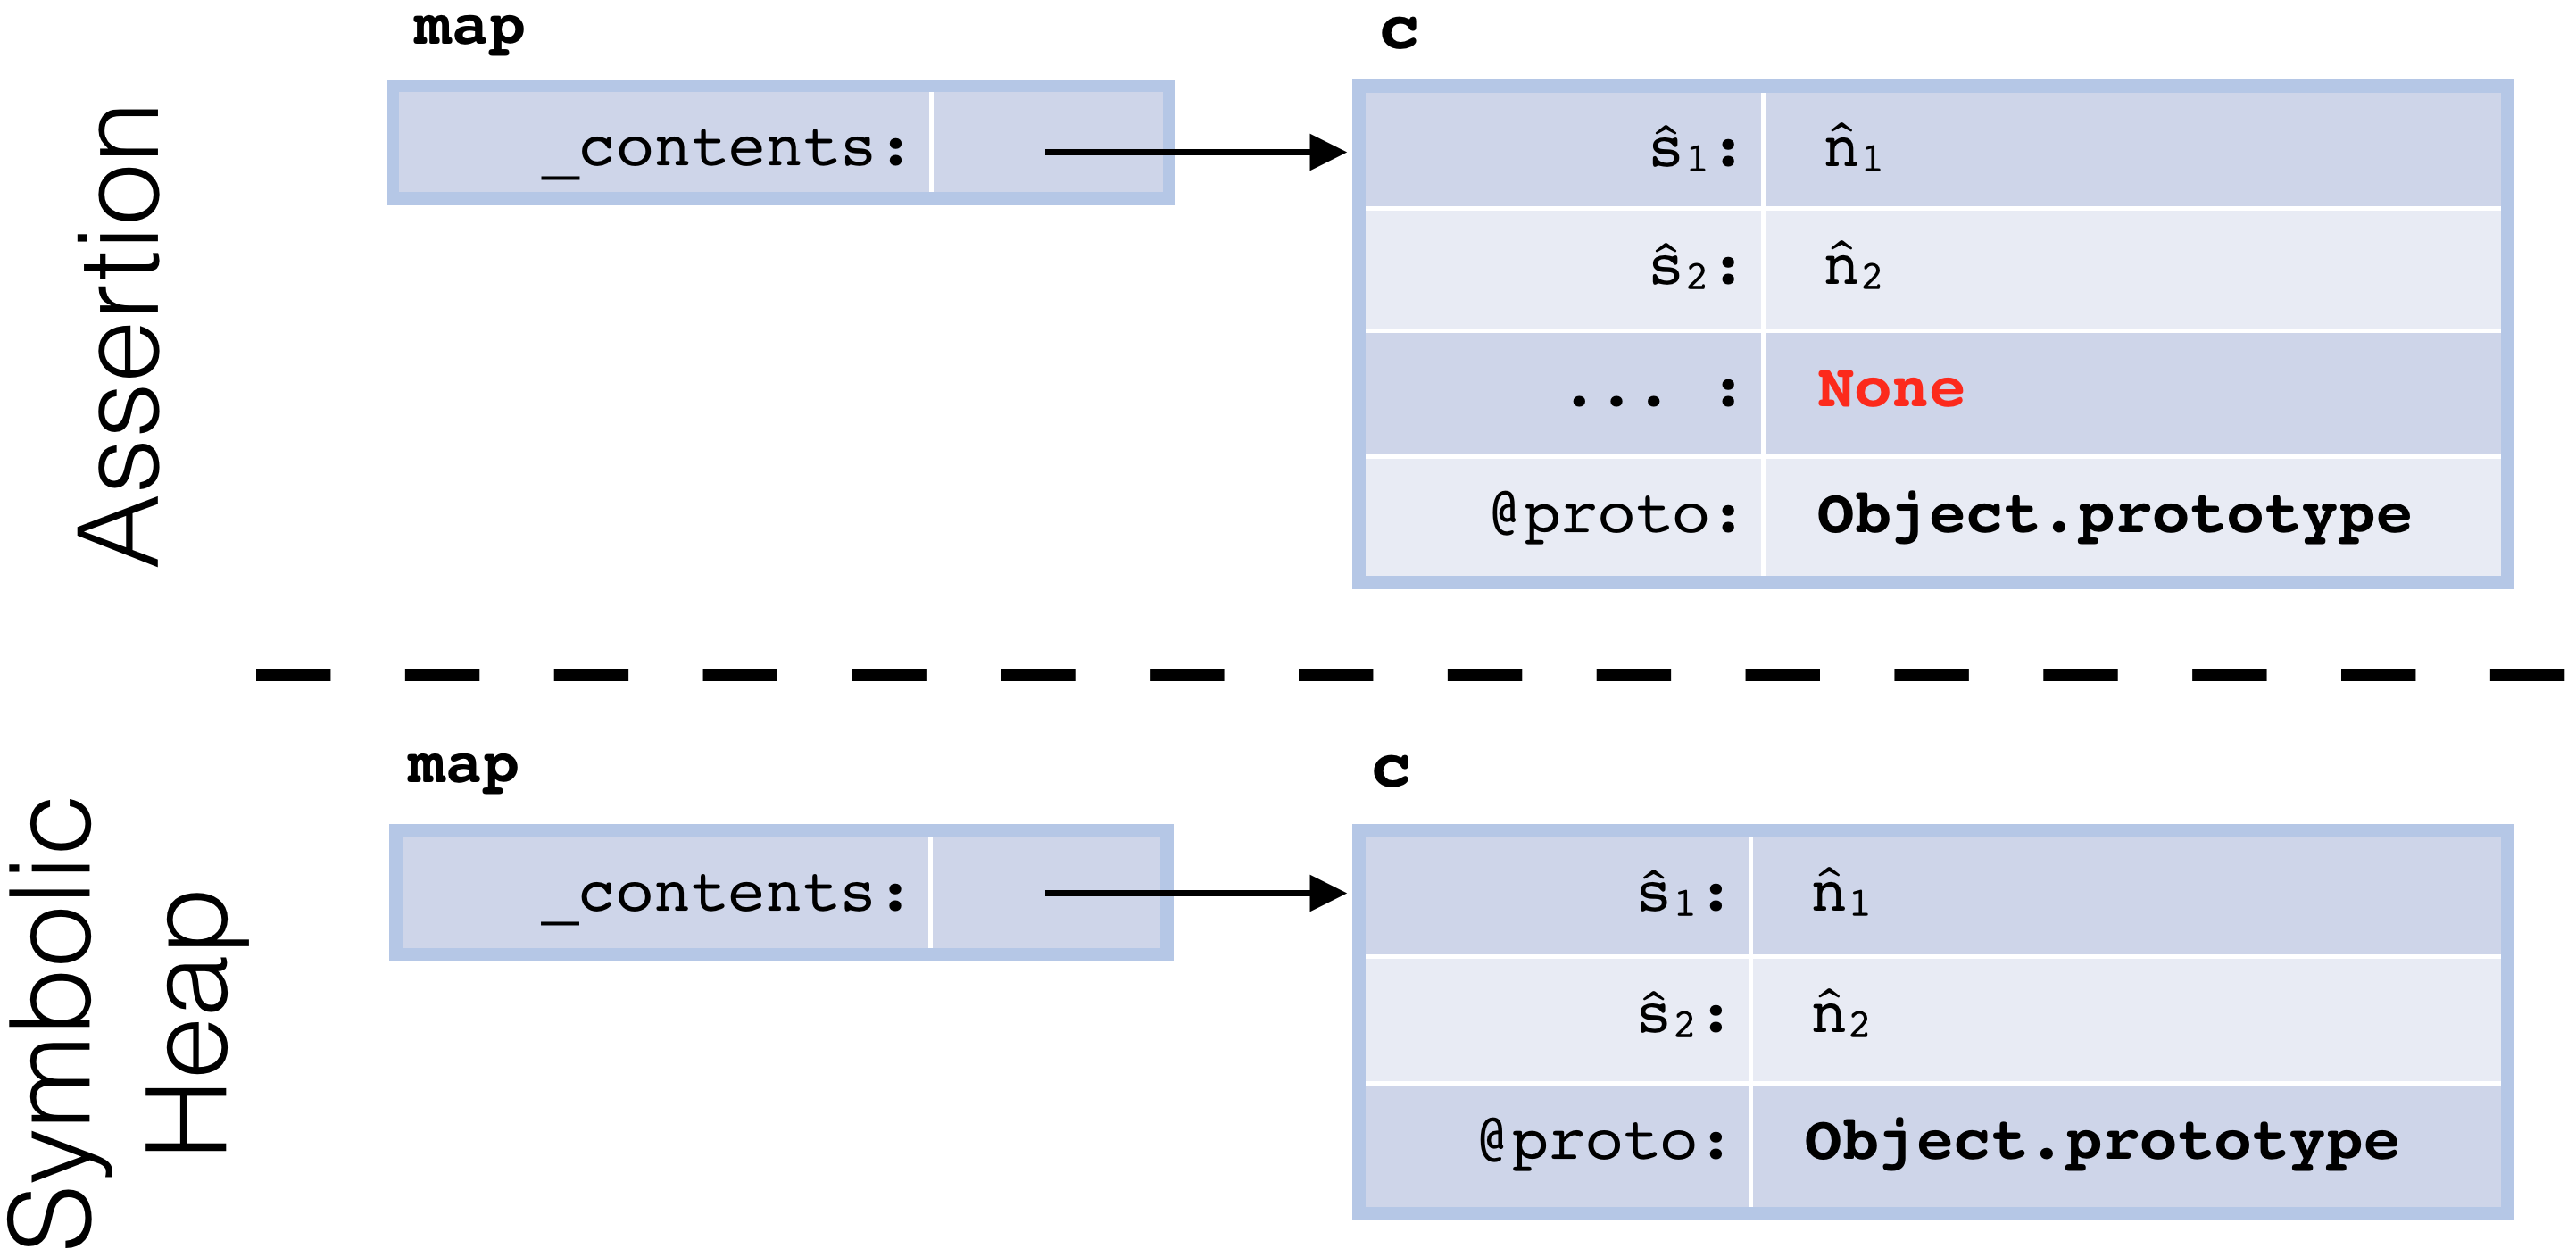
\includegraphics[width=0.29\textwidth]{figures/symbvsass.png}
%\vspace*{-0.3cm}
%\caption{Unfolded assertion {\scriptsize$\mathtt{Map(map, \{ (\hat{s}_1, \hat{n}_1), (\hat{s}_2, \hat{n}_2) \} )}$}}\label{fig:symb:state:versus:assertion}
%\label{fig:unfolded}
%\vspace*{-0.4cm}
%\end{wrapfigure}
%
%The \jsinline|ValidKey(k)| predicate captures the validity of a given key and holds \emph{iff} the corresponding JavaScript function \jsinline|validKey(k)| returns \jsinline|true|.
%In the definition of \jsinline|ValidKey|, we highlight in red a potential bug in the specification, already seen in the symbolic testing example.
%% source of errors on which we will focus shortly.
%
%To give a better intuition of how the \jsinline|Map| predicate works, we show the full unfolding of {\small$\mathtt{Map(map, \{ (k_1, v_1), (k_2, v_2) \} )}$} in Figure \ref{fig:symb:state:versus:assertion}. 
%
%\noindent
%\begin{minipage}{0.475\textwidth}
%\begin{displaymath} 
%{\scriptsize
%\hspace*{-0.2cm}
%\begin{array}{c}
%\left\{ {\begin{array}{c}
% \text{\texttt{Map(this, kvs -u- (k, v)) * ObjProtoF() *}} \\
% \text{\texttt{(this, "@proto") -> mp * MapProto(mp) * ...}}
%\end{array}} \right\} \\
%%
%\text{\bfseries \texttt{get(k)}} \\[0.2mm]
%%
%\left\{ {\begin{array}{c}
% \text{\texttt{Precondition * (ret = v)}} 
%\end{array}} \right\}
%\end{array}
%} 
%\end{displaymath}
%\end{minipage}
%\quad
%\begin{minipage}{0.48\textwidth}
%%
%\begin{displaymath} 
%{\scriptsize
%\begin{array}{c}
%\left\{ {\begin{array}{c}
% \text{\texttt{Map(this, kvs -u- (k, v')) * ObjProtoF() *}} \\
% \text{\texttt{(this, "@proto") -> mp * MapProto(mp) * ...}}
%\end{array}} \right\} \\
%%
%\text{\bfseries \texttt{put(k, v)}} \\[0.2mm]
%%
%\left\{ {\begin{array}{c}
% \text{\texttt{Map(this, kvs -u- (k, v)) * ObjProtoF() *}} \\
% \text{\texttt{(this, "@proto") -> mp * MapProto(mp) * ...}}
%\end{array}} \right\}
%\end{array}
%} 
%\end{displaymath}
%\end{minipage}
%
%\vspace{5pt}
%The predicate \jsinline|ObjProtoF()| describes the \jsinline|Object.prototype| object. It is needed because \jsinline|get| uses the \jsinline|hasOwnProperty| function, defined in \jsinline|Object.prototype|. 
%The predicate \jsinline|MapProto| specifies the resource of a valid map prototype: in particular, it defines the \jsinline|put|, \jsinline|get|, and \jsinline|validKey| methods.
%
%Given a JavaScript function, its separation logic specification, and the depth to which the unfold recursive predicates (non-recursive predicates are unfolded automatically), \cosette generates symbolic tests to verify that the function conforms to the specification up to that given depth.
%Now, if we forgot to state the part of the \jsinline|ValidKey(k)| predicate highlighted in red, that is, if we did not state that \jsinline|k <> "hasOwnProperty"|, the symbolic test generated for the specification of \jsinline|get| would fail for depth $\geq 1$, with the counter-model \jsinline|k = "hasOwnProperty"|, triggering the same bug previously described in the context of symbolic testing.

%\subsection{Catching \polish{procedure-local} bugs}
%
%The bug associated with the shadowing of the \jsinline|hasOwnProperty| property of \jsinline|Object.prototype| illustrates how a JavaScript library can be broken by only using its own functions. However, as JavaScript does not observe the frame property, there exists an additional class of bugs that can be triggered by the environment in which the library is run. These bugs expose how the library is not resilient against the possible frames and signal which properties of which objects must not be present in order for the library to behave correctly.
%
%To illustrate such bugs, recall the symbolic test from \S\ref{subsec:st}. This symbolic test creates an empty map on which it checks whether or not the behaviour of \jsinline|put| is correct. After catching the \jsinline|hasOwnProperty| bug, one might want to construct a more general test, starting from an arbitrary map. For this, one would need to use the \jsinline|Map| predicate from \S\ref{subsec:sdbf}:
%
%\begin{Verbatim}[fontsize=\footnotesize,commandchars=\\\{\}]
%         Map (m, kvs) := DataProp(m, "_contents", c) * JSObject(c) * 
%                           KVPairs(c, kvs) * first(kvs, keys) * emptyFields(c, keys)
%\end{Verbatim}
%
%\noindent as part of the initial state in which to run the symbolic test. Then, however, on execution of the test, when we reach the \jsinline|m.put(k, v)| command, we will get an error. The symbolic execution will not be able to determine if the property \jsinline|put|, which is supposed to be found in \jsinline|Map.prototype|, exists in the object~\jsinline|m| or not. This means that an environment can break the map library by putting into a map object the properties that are meant to be found in its prototype, and also that the specification of maps needs to be strengthened to forbid this explicitly:
%\begin{Verbatim}[fontsize=\footnotesize,commandchars=\\\{\}]
%   Map (m, kvs) := DataProp(m, "_contents", c) * JSObject(c) * 
%                     \textcolor{red}{((m, "get) -> none)} * \textcolor{red}{((m, "put") -> none)} * \textcolor{red}{((m, "validKey") -> none)} *
%                       KVPairs(c, kvs) * first(kvs, keys) * emptyFields(c, keys).
%\end{Verbatim}
%
%Bugs such as this will very rarely be caught by whole-program analyses, because there the entire state of the program is known and the test needs to be especially crafted with these bugs in mind. The reason that \cosette can catch them easily is because it is compositional and can run in partially described states.
